
\section{The likelihood-based reconstruction of the JUNO water-phase}
Super-Kamiokande~(SK) is the largest water Cherenkov detector in the world, with a water mass of 50 kilotons~\cite{SK}.
Building upon the liquid scintillator-Cherenkov combined track reconstruction technique developed for the MiniBooNE experiment~\cite{minibone}, SK collaboration has advanced a likelihood-based reconstruction method, utilizing PMT charge and time information~\cite{SKfiTQun}, named as fiTQun.  For JUNO water-phase, we have implemented targeted improvements to the fiTQun and extended its application to low-energy event reconstruction at the \si{MeV} scale.

\subsection{The Likelihood function}
FiTQun simultaneously determines particle types, vertex positions, momentums, event times.
In JUNO water-phase, we just need to determine the vertex position, momentums and event times.
The likelihood function of fiTQun is defined as:
\begin{equation}
	\log \mathcal{L}(\boldsymbol{x};{q},{t}) = \sum_{j \in \{q=0\}} \log P_j \bigl( q=0\bigm| \mu_j \bigr) + \sum_{i \in \{q>0\}} \log \bigl( f_{\mathrm{q}}\bigl( q_i \bigm| \mu_i \bigr) \bigr) + \sum_{i \in \{q>0\}} \log \bigl( f_{\mathrm{t}} \bigl( t_i \bigm| \boldsymbol{x} \bigr) \bigr)
\end{equation}
\begin{itemize}
	\item $\boldsymbol{x} = (t_0, x, y, z, p_x, p_y, p_z)$: Event vertex containing time $t_0$, position $(x,y,z)$, and momentum $(p_x,p_y,p_z)$.
	\item $\mu_i(\boldsymbol{x})$: Expected photoelectrons (PEs) at the $i$-th PMT, computed from the vertex $\boldsymbol{x}$.
	\item $q_i$: Charge observed at the $i$-th PMT, $\{q\}$ is the sequence of $q_i$, when $q_i=0$, the PMT is unhitted.
	\item $t_i$: Hit time of the $i$-th PMT, $\{t\}$ is the sequence of $t_i$.
\end{itemize}

The first term is the unhit likelihood, which is the probability of no hit in the PMT. The second term is the hit likelihood, which is the probability of detecting hits in the PMT. The third term is the time likelihood, which is the probability of detecting a hit at a certain time.

Since in the operation of the detector, only TQ information (time and charge) is recorded for low-energy events, waveform information is unavailable. At the same time only the first hit time can be obtained. Therefore, it is necessary to reformulate the likelihood to adopt a first-hit-time-based reconstruction approach. Xuewei Liu~et.al developed a first-principles-based reconstruction method using time-charge information or time-PE information in liquid scintillator detectors~\cite{Liu:2024cxo}. We adapt their methodology to reformulate the likelihood function for JUNO water-phase. In low-energy events, where each PMT typically detects only few photon, the number of hits can be directly approximated as NPE~($N_{PE}$). We can reformulate the likelihood function as:
\begin{equation}
	\log \mathcal{L}(\boldsymbol{x};{q},{t})= \sum_{j \in \{q=0\}}\log P_j \bigl( q=0\bigm| \mu_j \bigr)+\sum_{i \in \{q>0\}} \log \bigl( f_{\mathrm{q}}\bigl( 0 \bigm| \mu_{i,T_{low}}^{T_i} \bigr) * f_{\mathrm{t}}(T_i) * f_{\mathrm{q}}(N_{PE,i}-1|\mu_{i,T_{i}}^{T_{up}}) \bigr)
\end{equation}

In this case, we define the data taking as $[T_{low},T_{up}]$, and the first hit time of the $i$-th PMT as $T_{i}$, $\mu_{i,T_{low}}^{T_i}$ is the expected PEs in [$T_{low}$,${T_i}$], same as $\mu_{i,T_{i}}^{T_{up}}$.

\subsection{Response of the water-phase dector}
To compute the likelihood, we need to predict how many photons each PMT will detect when given a vertex. The more accurate the predictions are, the better the reconstruction performances. Therefore, we need a comprehensive understanding of the detector response and develop accurate models for it.
It naturally comes to mind that when a charged particle enters water, emits Cherenkov photons, and triggers the PMT, this process can be divided into two parts. One pertains to how Cherenkov light is emitted, while the other concerns how the Cherenkov photons propagate and are detected.

\subsubsection{The Cherenkov emission profile}
When a charged particle travels through a medium at a speed exceeding that of light, it emits Cherenkov photons within a specific solid angle range. The phenomenon arises from local polarization occurring along the charged particle's trajectory: when polarized molecules return to their ground state, they emit electromagnetic radiation. When the refractive index of the medium is $n$, and the speed of light in vacuum is $c_0$, the condition of particle speed~$v_p$ for Cherenkov emmision is $\beta=v_p/c_0>1/n$. When in pure water, whose refractive index is $n_w=1.333$, and the paitical is electron~($m_0=\SI{0.511}{MeV}$), the energy threthold is $E_{th}=m_0\times(\sqrt{1-1/n_w^2}-1)=\SI{0.262}{MeV}$. That means, only when the energy of electron is larger than \SI{0.262}{MeV}, the Cherenkov photons will emit.

The direction of Cherenkov photons can be discribed as: $\cos\theta=\frac{1}{\beta n_w}$ as Fig~\ref{Fig:Cherenkov_emmision} shown.

\begin{figure}
	\begin{center}
		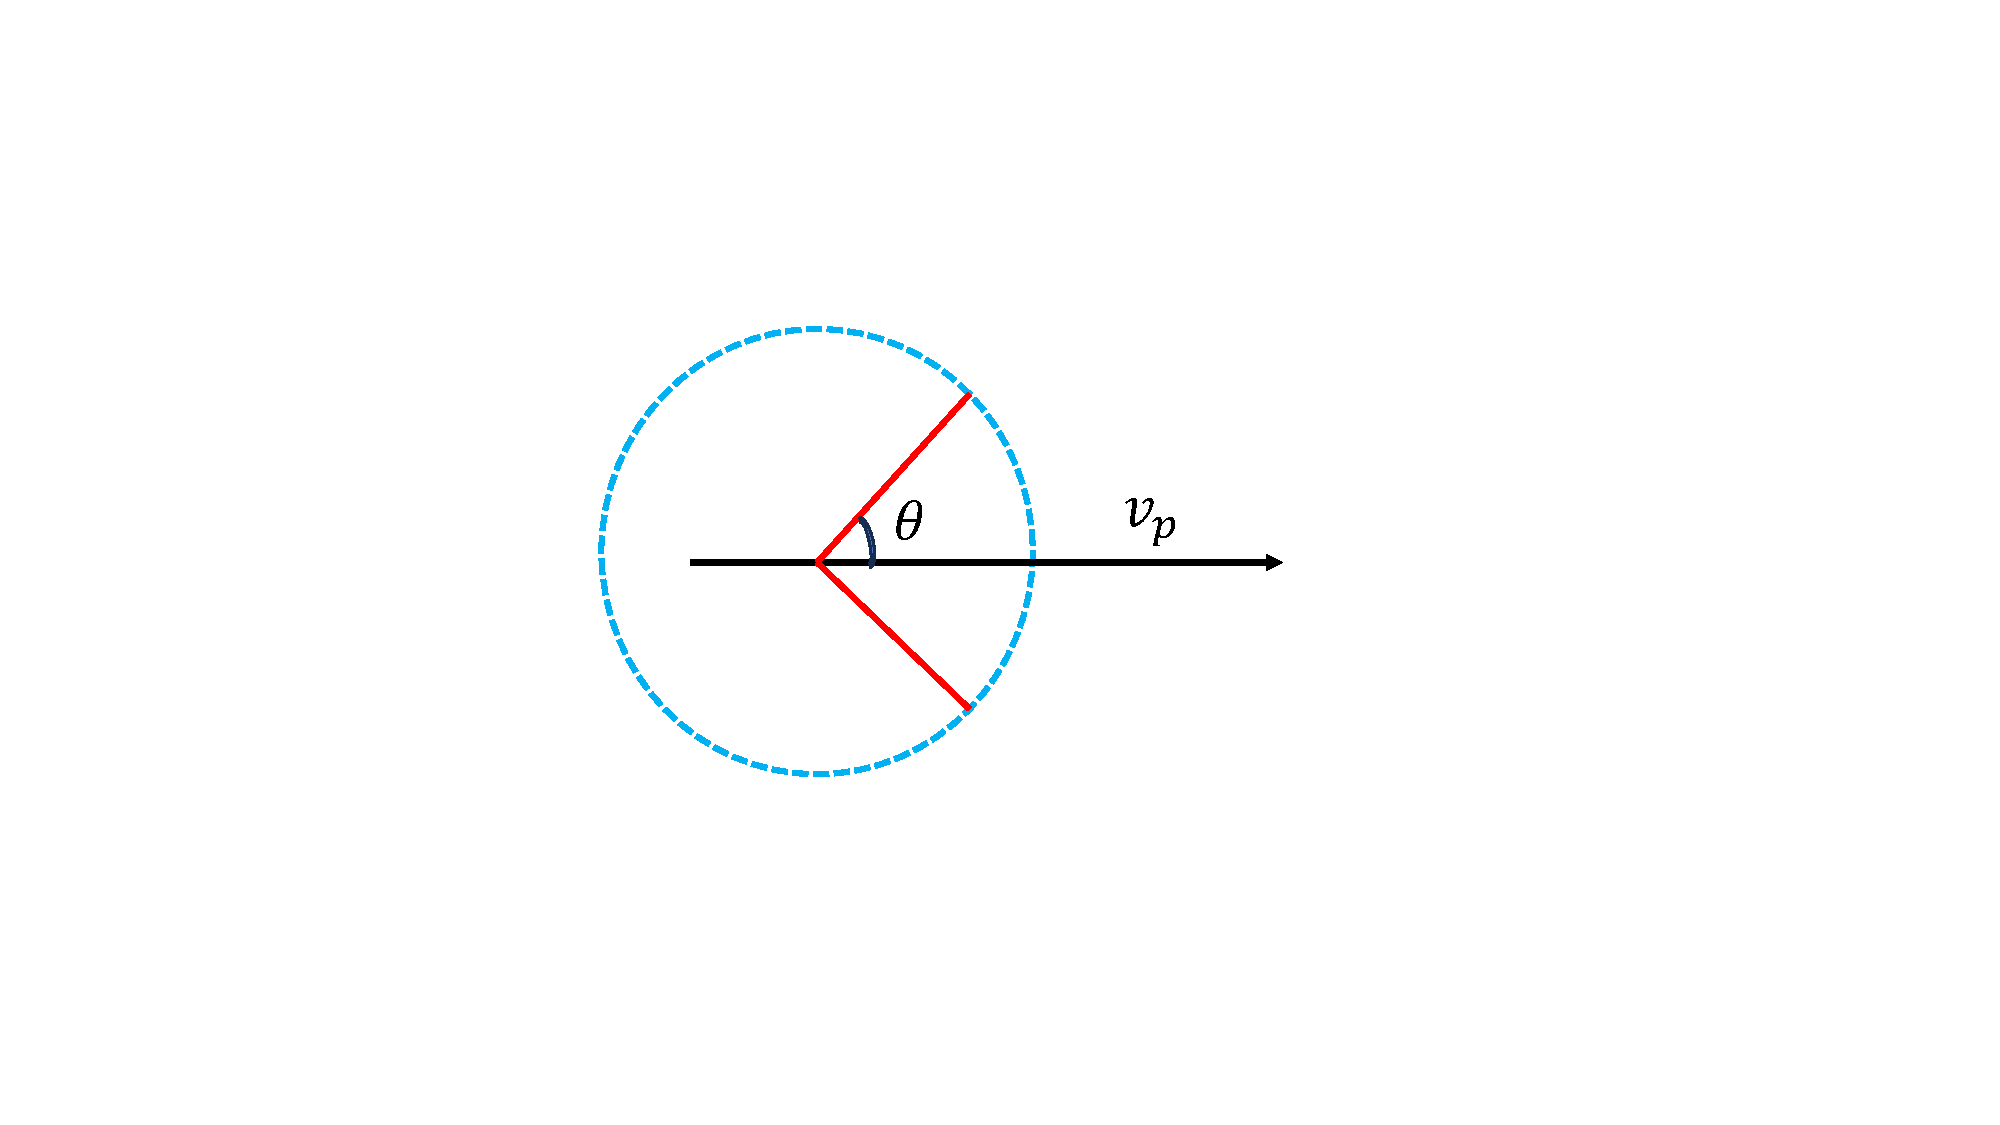
\includegraphics[height=6cm]{reconstruction/cherenkov_emission.pdf}
	\end{center}
	\caption{The direction of Cherenkov photons. $\theta$ is the angle between the photon emission direction and the direction of particle motion.}
	\label{Fig:Cherenkov_emmision}
\end{figure}

When in water, $\cos\theta\approxeq0.75$. We can use simulation to get the emmision profile of Cherenkov photons. We used JUNO software~(version: J24.2.0) for this simulation. Also, we consider the light yield of Cherenkov by simulating electron with momentum from \SI{2}{MeV} to \SI{30}{MeV}. Our simulation is based on JUNO software~(JUNOsw)~\cite{junosw}, and the version is J24.2.1. We simulated electrons with momenta ranging from 2 to 50 MeV, uniformly distributed within the detector, while their emission directions were randomly oriented.

We extended Dou Wei's angular coordinate definition method for liquid scintillator detectors~\cite{Dou:2022} to Cherenkov radiation detection by incorporating momentum direction degrees of freedom, resulting in the coordinate system illustrated in the figure.

\begin{figure}
	\begin{center}
		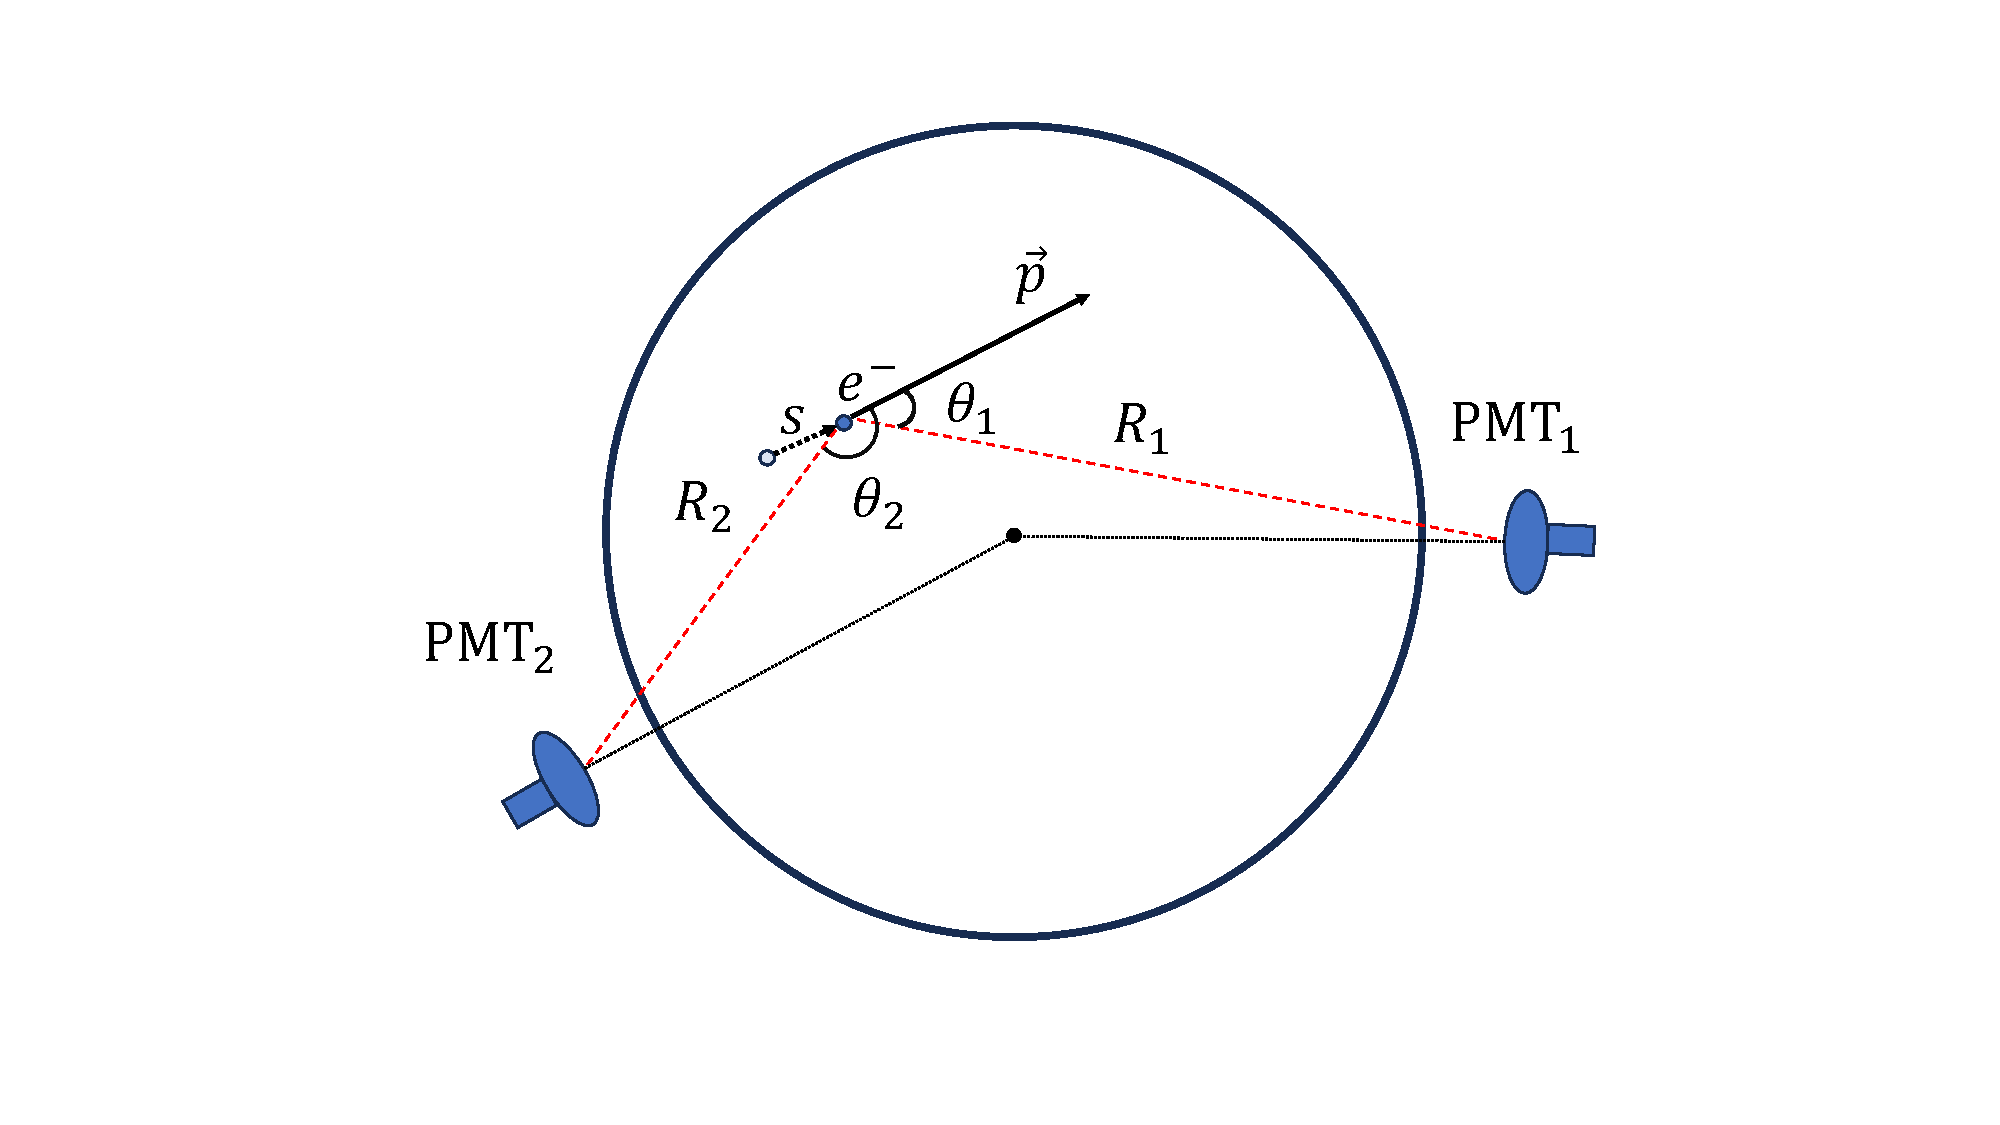
\includegraphics[height=6cm]{reconstruction/zuobiao.pdf}
	\end{center}
	\caption{Coordinate system definition: $\theta$ is the angle of the emission direction of Cherenkov photon and the incident direction of the electron, $s$ is the distance from the position where the particle emits light to its initial position. $R$ is the distance of PMT to the position of electron.}
	\label{Fig:Coordinate}
\end{figure}

In this simulation, we recorded the angles between the emission directions of all Cherenkov photons and the incident direction of the electron, and we do not care the photons are detected or not. Simultaneously, a crucial parameter is the distance between the photon generation point and the origin position of the charged particle.
\begin{itemize}
	\item From Fig~\ref{fig:thetaemmision}, most photons are emitted along the Cherenkov angle~($\cos\theta=0.75$), while a minority exhibit significant angular deviations from the electron's direction. When calculating the emission angle distribution, it must be analyzed separately for different particle energies rather than applying a single angular distribution to electrons of all energies.
	\item From Fig~\ref{fig:semmision}, as the particle moves, Cherenkov photons emitted along the initial segment of its trajectory exhibit a uniform distribution. When the particle's velocity significantly decreases, photon emission drops markedly, with the vast majority of photons being emitted within the first half of the trajectory.
	\item From Fig~\ref{fig:tsemmision}, after traveling some distance, the probability of photons deviating from the Cherenkov angle gradually increases due to multiple scattering. As illustrated in the figure, when electrons undergo multiple scattering, their direction changes significantly, as Fig~\ref{fig:multipleScattering} shown. However, when calculating the Cherenkov emission angle, we still use the initial incident direction, thereby producing photons emitted at angles far from the ideal Cherenkov angle.
	\item In this case, we get the Cherenkov emmision profile~($g(p,s,\theta)$) which describes the proportion of Cherenkov photons emitted at specific locations and directions along the trajectory of a charged particle with a given energy, relative to the total number of emitted photons. For the convenience of research, we use momentum~($p$) instead of energy~($E$).
\end{itemize}

\begin{figure}[h]
	\centering
	\begin{subfigure}{0.45\textwidth}
		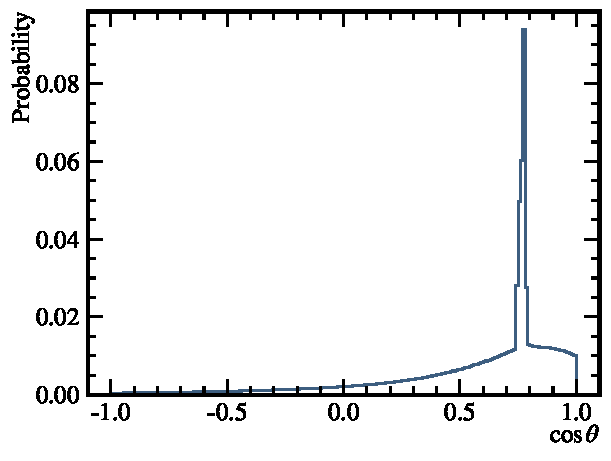
\includegraphics[page=1,width=\textwidth]{reconstruction/emmisionProfile/2.pdf}
		\caption{\SI{2}{MeV} electron}
		\label{fig:theta2mev}
	\end{subfigure}
	\hfill
	\begin{subfigure}{0.45\textwidth}
		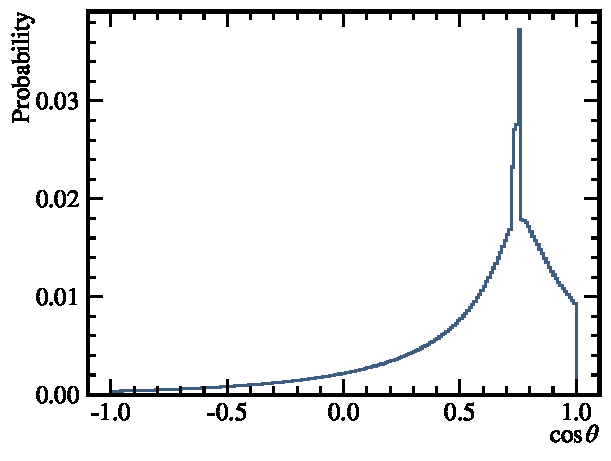
\includegraphics[page=1,width=\textwidth]{reconstruction/emmisionProfile/5.pdf}
		\caption{\SI{5}{MeV} electron}
		\label{fig:theta5mev}
	\end{subfigure}

	\vspace{\baselineskip}

	\begin{subfigure}{0.45\textwidth}
		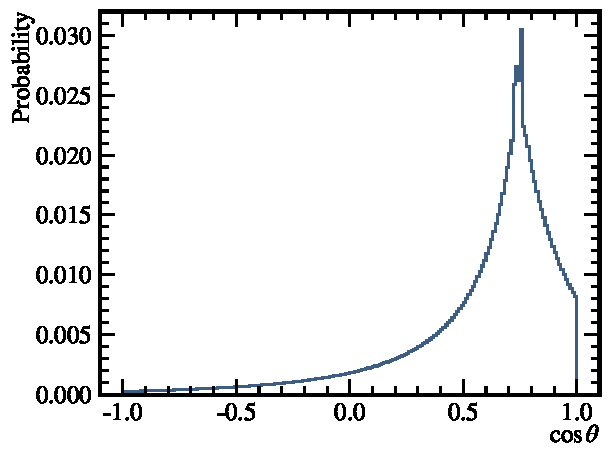
\includegraphics[page=1,width=\textwidth]{reconstruction/emmisionProfile/10.pdf}
		\caption{\SI{10}{MeV} electron}
		\label{fig:theta10mev}
	\end{subfigure}
	\hfill
	\begin{subfigure}{0.45\textwidth}
		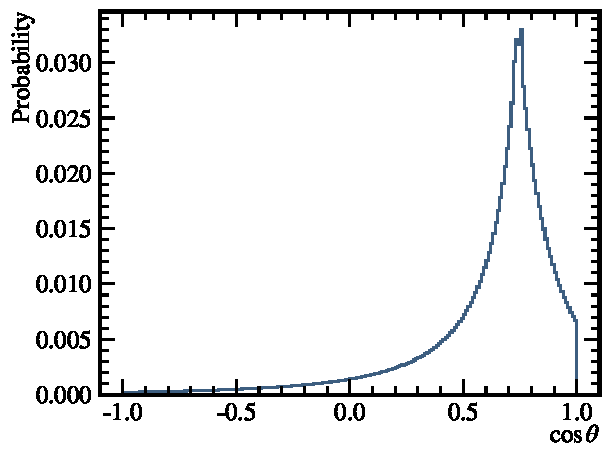
\includegraphics[page=1,width=\textwidth]{reconstruction/emmisionProfile/20.pdf}
		\caption{\SI{20}{MeV} electron}
		\label{fig:theta20mev}
	\end{subfigure}
	\caption{The relationship of emission probability with $\cos\theta$.}
	\label{fig:thetaemmision}
\end{figure}

\begin{figure}[h]
	\centering
	\begin{subfigure}{0.45\textwidth}
		\includegraphics[page=2,width=\textwidth]{reconstruction/emmisionProfile/2.pdf}
		\caption{\SI{2}{MeV} electron}
		\label{fig:s2mev}
	\end{subfigure}
	\hfill
	\begin{subfigure}{0.45\textwidth}
		\includegraphics[page=2,width=\textwidth]{reconstruction/emmisionProfile/5.pdf}
		\caption{\SI{5}{MeV} electron}
		\label{fig:s5mev}
	\end{subfigure}

	\vspace{\baselineskip}

	\begin{subfigure}{0.45\textwidth}
		\includegraphics[page=2,width=\textwidth]{reconstruction/emmisionProfile/10.pdf}
		\caption{\SI{10}{MeV} electron}
		\label{fig:s10mev}
	\end{subfigure}
	\hfill
	\begin{subfigure}{0.45\textwidth}
		\includegraphics[page=2,width=\textwidth]{reconstruction/emmisionProfile/20.pdf}
		\caption{\SI{20}{MeV} electron}
		\label{fig:s20mev}
	\end{subfigure}
	\caption{The relationship of emission probability with $s$.}
	\label{fig:semmision}
\end{figure}


\begin{figure}[h]
	\centering
	\begin{subfigure}{0.45\textwidth}
		\includegraphics[page=3,width=\textwidth]{reconstruction/emmisionProfile/2.pdf}
		\caption{\SI{2}{MeV} electron}
		\label{fig:ts2mev}
	\end{subfigure}
	\hfill
	\begin{subfigure}{0.45\textwidth}
		\includegraphics[page=3,width=\textwidth]{reconstruction/emmisionProfile/5.pdf}
		\caption{\SI{5}{MeV} electron}
		\label{fig:ts5mev}
	\end{subfigure}

	\vspace{\baselineskip}

	\begin{subfigure}{0.45\textwidth}
		\includegraphics[page=3,width=\textwidth]{reconstruction/emmisionProfile/10.pdf}
		\caption{\SI{10}{MeV} electron}
		\label{fig:ts10mev}
	\end{subfigure}
	\hfill
	\begin{subfigure}{0.45\textwidth}
		\includegraphics[page=3,width=\textwidth]{reconstruction/emmisionProfile/20.pdf}
		\caption{\SI{20}{MeV} electron}
		\label{fig:ts20mev}
	\end{subfigure}
	\caption{The relationship of emission probability with $s$ and $\cos\theta$.}
	\label{fig:tsemmision}
\end{figure}

\begin{figure}
	\begin{center}
		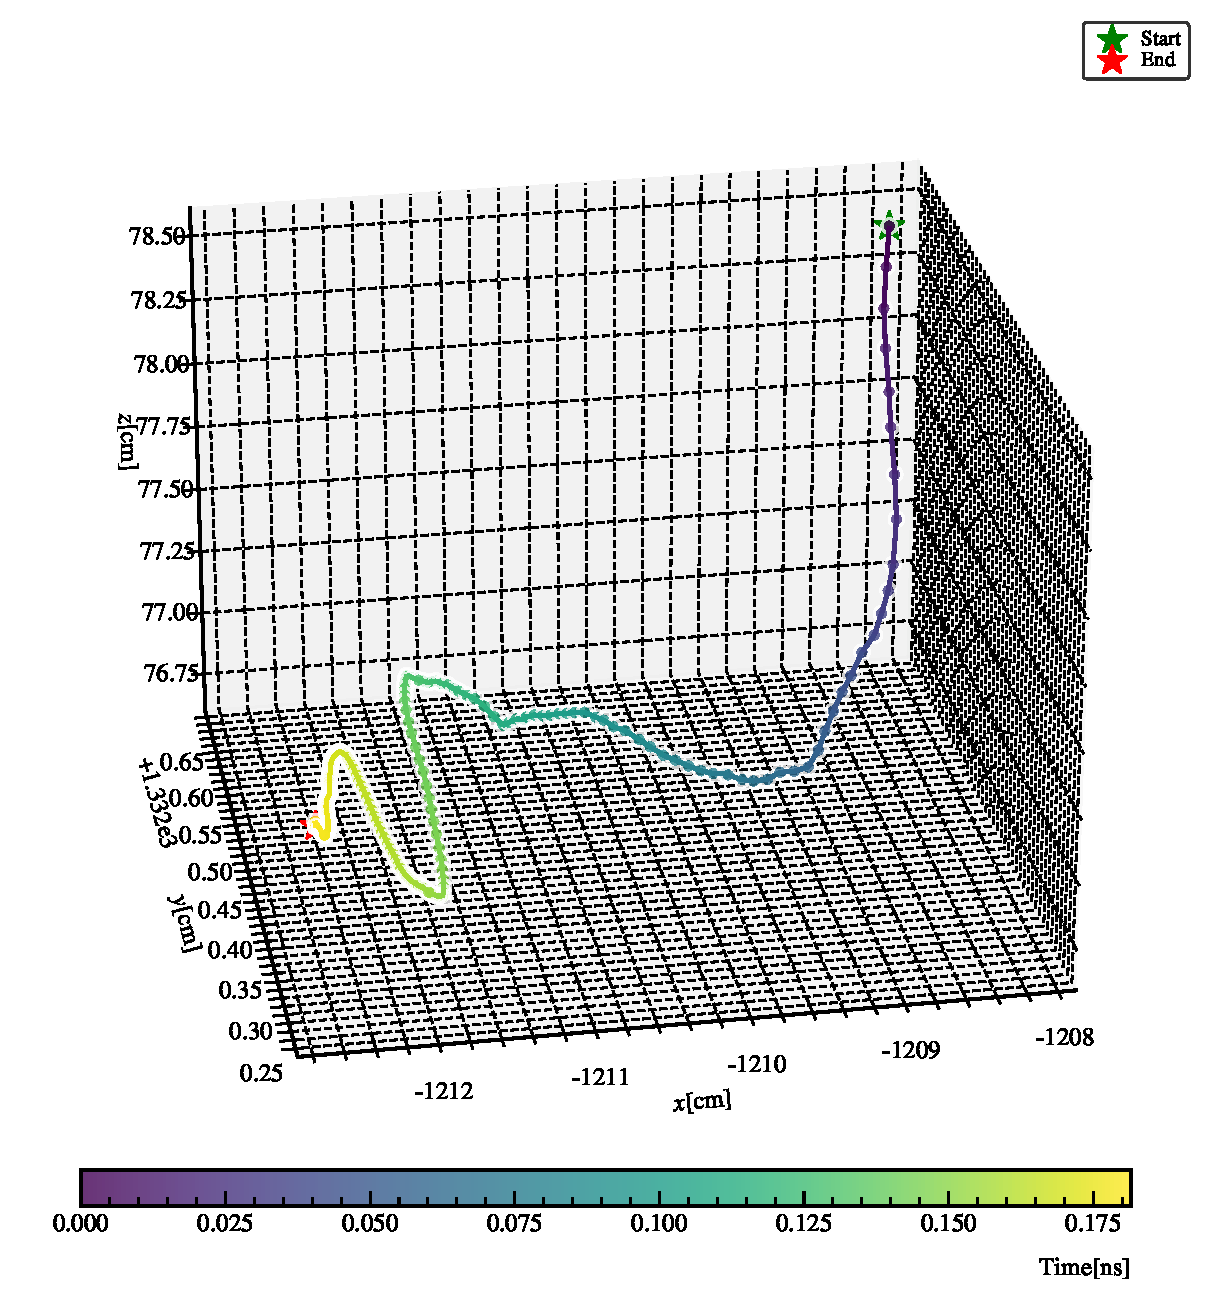
\includegraphics[width=0.8\textwidth]{reconstruction/emmisionProfile/multiscatter.pdf}
	\end{center}
	\caption{An example of a \SI{10}{MeV} electron undergoing multiple scattering.}
	\label{fig:multipleScattering}
\end{figure}

Through Gaussian fitting as shown in Fig~\ref{fig:yield_gauss_fit} in simulation, we obtain the total number of photons emitted at various energies and calculate the Cherenkov photon yield. After linear fitting, we obtain the relationship between light yield and momentum: $\phi(p)=1182\times p-956$.
\begin{figure}[h]
	\centering
	\begin{subfigure}{0.45\textwidth}
		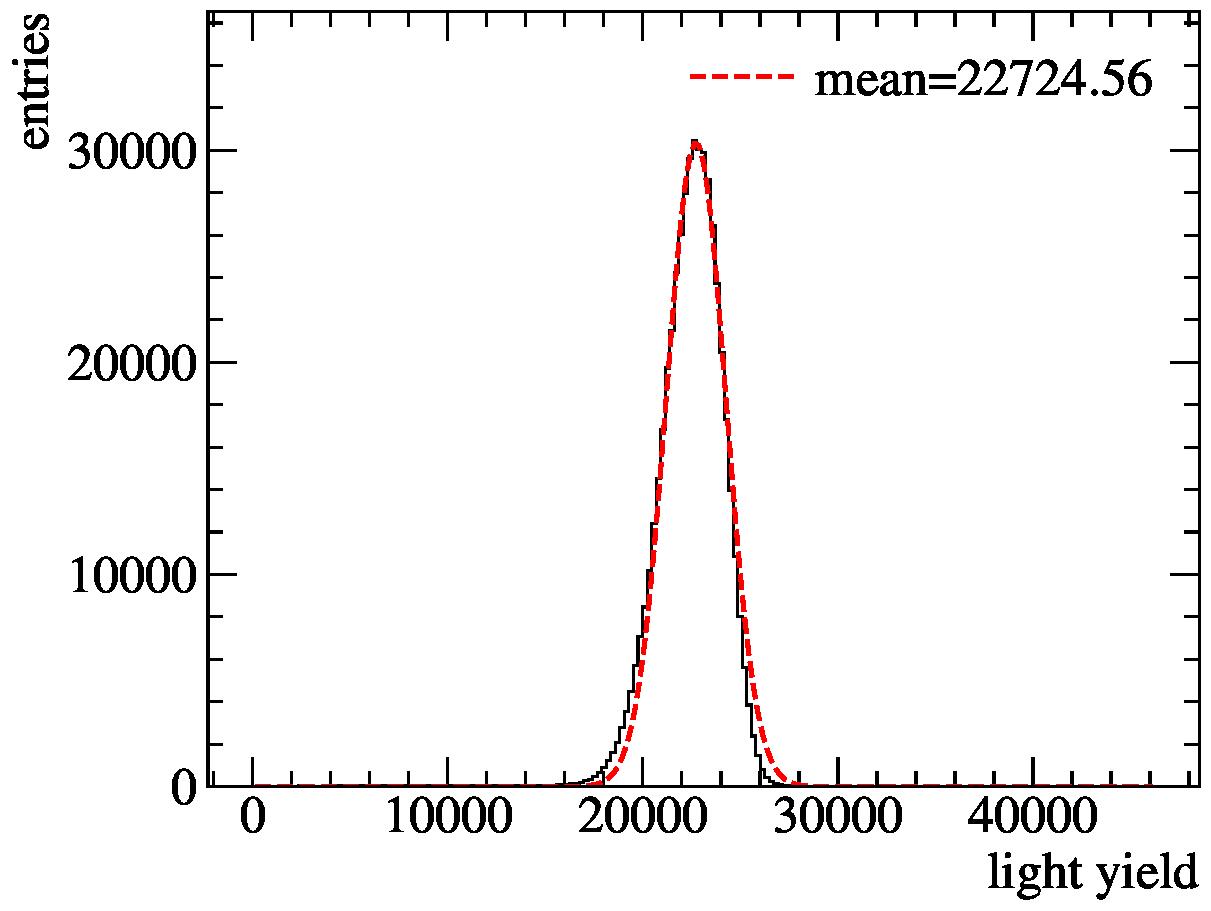
\includegraphics[width=\textwidth]{reconstruction/emmisionProfile/yield_gauss_fit_20.pdf}
		\caption{An example of Gaussian fit for light yield.}
		\label{fig:yield_gauss_fit}
	\end{subfigure}
	\hfill
	\begin{subfigure}{0.45\textwidth}
		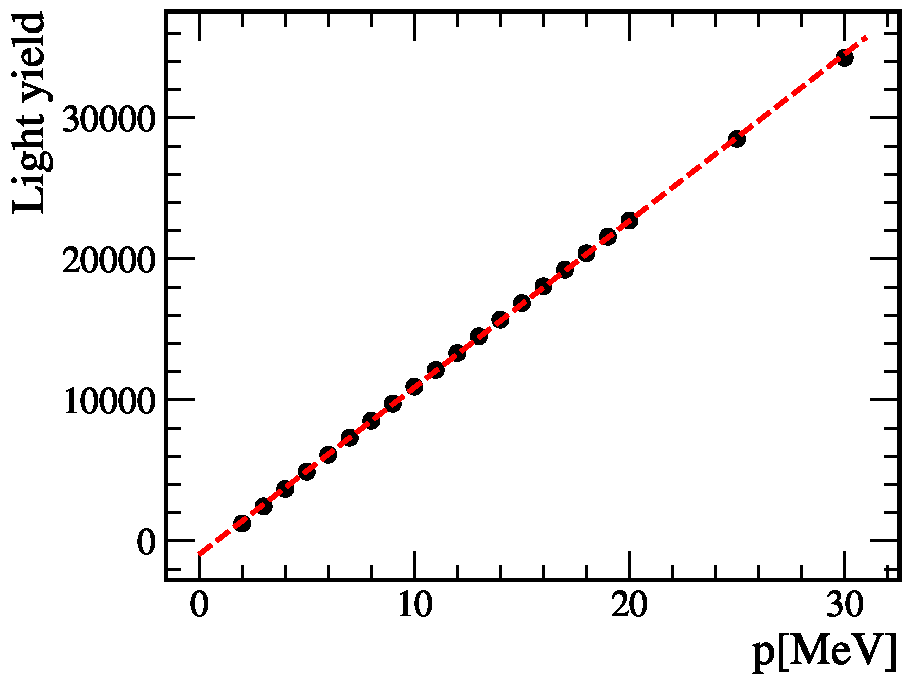
\includegraphics[width=\textwidth]{reconstruction/emmisionProfile/phip.pdf}
		\caption{\SI{5}{MeV} electron}
		\label{fig:yield_fit}
	\end{subfigure}
	\caption{The relationship of emission probability with $s$ and .}
\end{figure}

\subsubsection{The calculation of direct light}
After establishing the coordinate system, we can readily determine the number of photons received by a specific PMT when an electron is incident.
\begin{equation}
	\mu_{\mathrm{dir}}=\int ds g(p,s,\cos\theta)\phi(p)\Omega(R)T(R)\epsilon(\eta)
	\label{equ:directLight}
\end{equation}
\begin{itemize}
	\item $R$ is the distance between the position of electron and the PMT.
	\item $\Omega(R)$ is the solid angle factor of PMT.
	\item $T(R)$ is the light transmission factor.
	\item $\epsilon(\eta)$ is the PMT angular acceptance of PMT, and $\eta$ is the incident angle of light when captured by PMT.
\end{itemize}

\paragraph{The solid angle factor}
The main PMTs employed in JUNO are 20-inch with a radius of $a=SI{0.622}{m}$. And we can calculate the solid angle of PMT by Eq.~\eqref{equ:solid}.
\begin{equation}
	\Omega(R)=\frac{\pi a^2}{4\pi(R^2+a^2)}\times (4\pi)=\frac{\pi a^2}{R^2+a^2}
	\label{equ:solid}
\end{equation}
This approximation remains valid only when PMTs are sufficiently distant from the particle. In JUNO, PMTs are mounted at around \SI{19.5}{m} , while our region of interest lies within \SI{17.7}{m}. Based on SK's experience, the approximation holds effectively at radial distances $R > \SI{1.5}{m}$.

\paragraph{The transmission factor}
In our work, we just use Eq.~\eqref{eq:att}, and the attenuation length $L^{a}$ is \SI{75}{m}.
\begin{equation}
	T(R) = \exp(-R/L^{a})
	\label{eq:att}
\end{equation}

\paragraph{PMT angular accptance}


\subsection{The Fast reconstruction~(FRE) of the JUNO water-phase}
In the original fiTQun, the probability calculation for the charge term required generating extensive lookup tables to model. To streamline computations, we simplified the charge term by discretizing the charge $q$ into the number of photoelectrons~($N_{\mathrm{PE}}$).
In parallel, we utilize the first hit time of each PMT for reconstruction. This approach prioritizes the earliest detected photon arrival time at each PMT, which typically carries the most direct geometric and temporal information about the particle interaction. Based on the first-principles derivation of charge-time joint reconstruction in liquid scintillator detectors by Xuewei Liu et al.~\cite{xuewei}, we adapted their methodology to reformulate the likelihood function into Eq.~\ref{eq:likelihood}.
\section{The evaluation of reconstructions}
\subsection{The parameters used in the reconstruction}
\subsection{The reconstruction goodness of reconstruction}
The goodness of vertex is defined as the
\subsection{In the dector simulation}
\subsection{In the electronic simulation}
\subsection{The \ce{AmC} and \ce{AmBe} calibrations in water-phase}
Despite utilizing GPU acceleration for the reconstruction algorithms, we still face challenges in fully reconstructing all events. To reduce the data volume, we apply additional filtering during the fast reconstruction stage to remove dark noise-triggered events and events originating from PMT surface radioactivity outside the fiducial volume.
Let us use Run~3671 in which the \ce{AmBe} source is placed at $(0,0,-10)$\si{m} as an example to illustrate. Additionally, Run 3677, conducted under identical configuration conditions without deploying a calibration source, was selected as the background run.
\subsubsection{The reconstruction result of LFR}


\subsection{The combination of the two reconstruction algorithms}
\subsubsection{The events selected from the fast reconstruction}
